\begin{theo}[Wederzijdse inductie]{Wederzijdse inductie}
    \begin{minipage}{.78\textwidth}
        Als twee spoelen nabij elkaar plaatst worden, zoals in de figuur, dan zal een veranderende stroom in de ene, 
        een emf induceren in de andere. Dus: geïnduceerde emf in een spoel is enevredig met de snelheid van de stroomverandering
        in de andere. Dit noemt men \textbf{wederzijdse inductie} $M$, we noteren
        \begin{equation*}
            M_{21} = \dfrac{N_{2}\Phi_{21}}{I_{1}} 
        \end{equation*}
        met $M_{21}$ de wederzijdse inductiecoefficient en $\Phi_{21}$ de magnetische flux doorheen spoel 2 tegenover de stroom in spoel 1.
        We kunnen dit mengen met de wet van Faraday
    \end{minipage}
    \begin{minipage}{.18\textwidth}
        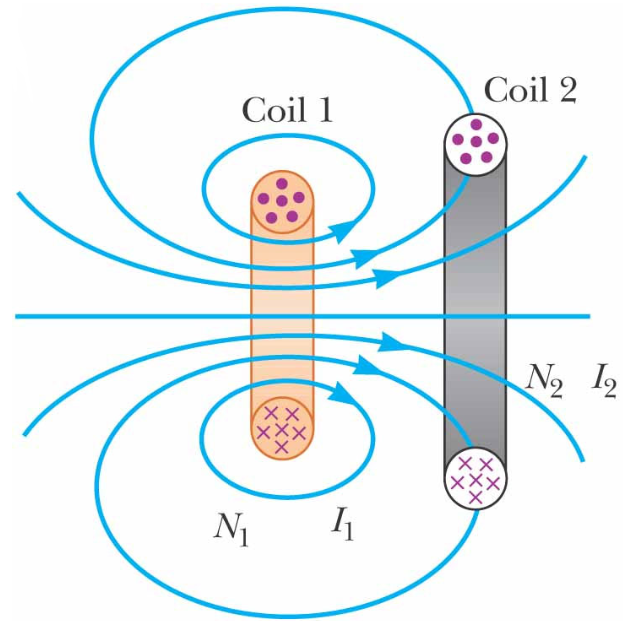
\includegraphics[scale=0.3]{Images/Magnetisme/WederzijdseInductie}
    \end{minipage}
    \begin{equation*}
        \mathcal{E}_{2} = - N_{2}\dfrac{d\Phi_{21}}{dt} = - M_{21}\dfrac{dI_{1}}{dt}
    \end{equation*}
    waarbij nu de verandering in stroom in spoel 1 hebben verbonden aan de emf dat het induceert in spoel 2.  In de algemene situatie is 
    $M = M_{12} = M_{21}$.
\end{theo}

% \begin{theo}[Wederzijdse inductie]{Wederzijdse inductie}
%     \begin{minipage}{.78\textwidth}
%         Als twee spoelen dicht bij elkaar worden geplaatst, zoals in de figuur, zal een veranderende stroom in de ene spoel een elektromotorische kracht (emf) induceren in de andere spoel. Met andere woorden, de geïnduceerde emf in een spoel is evenredig met de snelheid van de stroomverandering in de andere spoel. Dit staat bekend als \textbf{wederzijdse inductie} $M$, waarbij we noteren:
%         \begin{equation*}
%             M_{21} = \dfrac{N_{2}\Phi_{21}}{I_{1}} 
%         \end{equation*}
%         Hierbij staat $M_{21}$ voor de wederzijdse inductiecoëfficiënt en $\Phi_{21}$ voor de magnetische flux door spoel 2 als gevolg van de stroom in spoel 1.
%         Dit kan worden gecombineerd met de wet van Faraday.
%     \end{minipage}
%     \begin{minipage}{.18\textwidth}
%         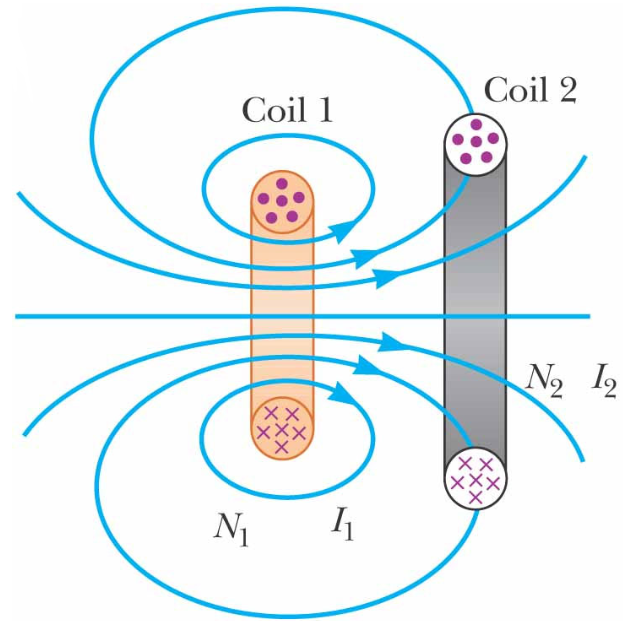
\includegraphics[scale=0.3]{Images/Magnetisme/WederzijdseInductie}
%     \end{minipage}
%     \begin{equation*}
%         \mathcal{E}_{2} = - N_{2}\dfrac{d\Phi_{21}}{dt} = - M_{21}\dfrac{dI_{1}}{dt}
%     \end{equation*}
%     Hiermee verbinden we de verandering in stroom in spoel 1 met de emf die het induceert in spoel 2. In de algemene situatie is $M = M_{12} = M_{21}$.
% \end{theo}


% \begin{app}[Wederzijdse inductie van een solenoïde en een spoel]{Wederzijdse inductie van een solenoïde en een spoel}
%     De solenoïde is opeengepakt, dus kunnen we veronderstellen dat alle magnetische flux in de solenoïde blijft in de tweede spoel.
%     We weten dam wat de flux door deze spoel is, namelijk
%     \begin{equation*}
%         \Phi_{21} = BA = \mu_{0}\dfrac{N_{1}}{\ell}I_{1}A
%     \end{equation*}
%     en de wederzijdse inductiecoëfficient
%     \begin{equation*}
%         M = \dfrac{N_{2}\Phi_{21}}{I_{1}} = \mu_{0}\dfrac{N_{1}N_{2}}{\ell}A
%     \end{equation*}
%     waarbij we zien dat deze enkel afhangt van de geometrie van het systeem.
% \end{app}

\begin{app}[Wederzijdse inductie van een solenoïde en een spoel]{Wederzijdse inductie van een solenoïde en een spoel}
    De solenoïde is compact, dus kunnen we aannemen dat alle magnetische flux in de solenoïde blijft en door de tweede spoel gaat.
    We weten dan wat de flux door deze spoel is, namelijk
    \begin{equation*}
        \Phi_{21} = BA = \mu_{0}\dfrac{N_{1}}{\ell}I_{1}A
    \end{equation*}
    en de wederzijdse inductiecoëfficiënt is
    \begin{equation*}
        M = \dfrac{N_{2}\Phi_{21}}{I_{1}} = \mu_{0}\dfrac{N_{1}N_{2}}{\ell}A
    \end{equation*}
    waaruit blijkt dat deze alleen afhankelijk is van de geometrie van het systeem.
\end{app}


\begin{theo}[Zelfinductie]{Zelfinductie}
    De magnetische flux $\Phi_{B}$ door een spoel met $N$ windingen (of eenderwelke kring) is evenredig met de stroom $I$ die erdoor vloeit, dus we definiëren de \textbf{zelfinductie} $L$ als
    \begin{equation*}
        L = \dfrac{N\Phi_{B}}{I}
    \end{equation*}
    Dus de geïnduceerde emf $\mathcal{E}$ in een spoel met zelfinductie $L$ is, volgens de wet van Faraday, gelijk aan
    \begin{equation*}
        \mathcal{E} = -N\dfrac{d\Phi_{B}}{dt }= - L\dfrac{dI}{dt}
    \end{equation*}
    \vspace{-0.3cm}
\end{theo}

\newpage

\begin{theo}[Energie opgeslagen in een magnetisch veld]{Energie opgeslagen in een magnetisch veld}
    Wanneer een inductor met zelfinductie $L$ een stroom $I$ heeft, die verandert met een snelheid $dI/dt$, dan is de energie die 
    gelever wordt aan de inductor gelijk aan 
    \begin{equation*}
        P = \mathcal{E}I = -LI\dfrac{dI}{dt}
    \end{equation*}
    De hoeveelheid arbeid $dW$ geleverd aan de inductor in een tijd $dt$ is gelijk aan
    \begin{equation*}
        dW = Pdt = -LIdI
    \end{equation*}
    De energie die opgeslagen is in het magnetisch veld van de inductor is gelijk aan de energie die geleverd is aan de inductor
    \begin{equation*}
        U = \int dW = \int Pdt = \int_{0}^{I} -LIdI = \dfrac{1}{2}LI^{2}
    \end{equation*}
    wat heel vergelijkbaar is aan de formule voor de energie opgeslagen in een condensator, namelijk: $U_{C} = \frac{1}{2}C(\Delta V)^{2}$. 
    Net zoals de energie in een condensator zich bevindt in het elektrisch veld tussen de platen,bevindt de energie in een inductor zich in het magnetisch veld binnenin de spoel.
\end{theo}

\begin{vrg}[Energiedichtheid]{Energiedichtheid}   
    \vspace{-0.3cm}
    \def\arraystretch{2}
    \centering
    \begin{tabular}{c|c}
        Energiedichtheid van een elektrisch veld & Energiedichtheid van een magnetisch veld \\[-0.35cm]
        van een spoel met zelfinductie $L$ en stroom $I$ & van een condensator met capaciteit $C$ en spanning $V$ \\ \hline
        $U_{E} = \dfrac{1}{2}\epsilon_{0}E^{2}$ & $U_{B} = \dfrac{1}{2}\mu_{0}B^{2}$ \\
    \end{tabular}
\end{vrg}

\begin{theo}[RL-kringen]{RL-kringen}
    \vspace{-0.5cm}
    \begin{minipage}{.66\textwidth}
        We sluiten de schakelaar en we passen de tweede wet van Kirchhoff toe op de kring. We krijgen
        \begin{equation*}
            V_{0} - IR - \mathcal{E} = V_{0} - IR - L\dfrac{dI}{dt} = 0
        \end{equation*}
        We kunnen dit herwerken tot een differentiaalvergelijking
        \begin{equation*}
            L\dfrac{dI}{dt} + RI = V_{0}
        \end{equation*}
        wat we oplossen tot 
        \begin{equation*}
            I(t) = \dfrac{V_{0}}{R}\left(1 - e^{\tfrac{-t}{\tau}}\right)
        \end{equation*} 
    \end{minipage}
    \begin{minipage}{.3\textwidth}
        \hspace{0.5cm}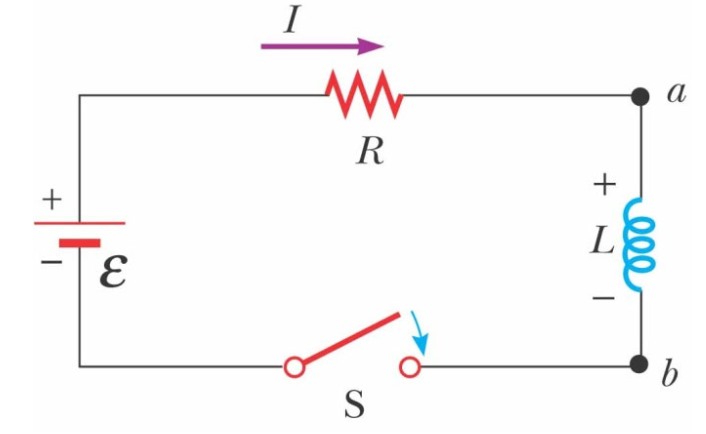
\includegraphics[scale = 0.35]{Images/Magnetisme/RLKring}
        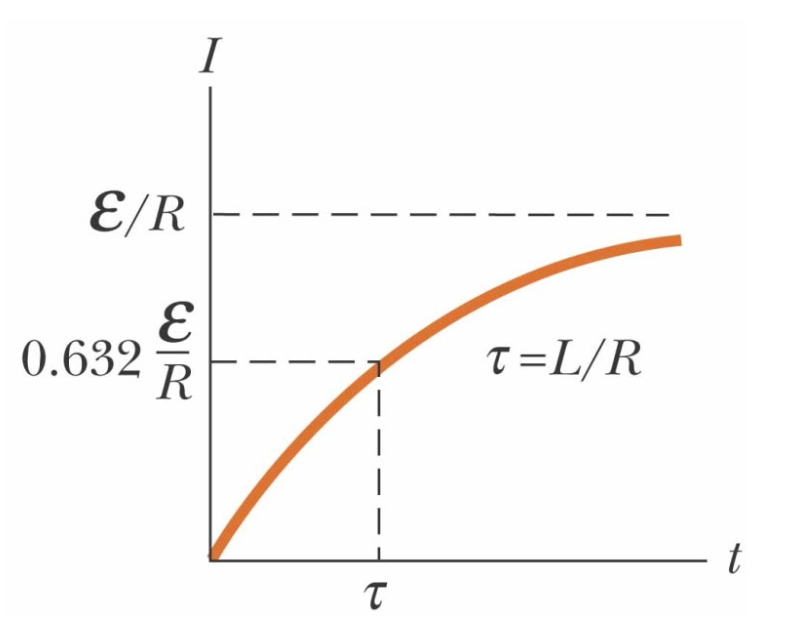
\includegraphics[scale = 0.35]{Images/Magnetisme/RLKringGraph.png}
    \end{minipage}

    \noindent met $\tau = \tfrac{L}{R}$. We zien dat de stroom initieel snel stijgt en dan afvlakt geleidelijk nabij $\tfrac{\mathcal{E}}{R}$.
\end{theo}

\newpage

\begin{theo}[Elektromagnetische oscillaties in LC-kringen]{Elektromagnetische oscillaties in RL-kringen}
    \vspace{-0.2cm}
    \begin{minipage}{.73\textwidth}
        We bekijken nu een kring met een inductor met inductantie $L$ en een condensator met capaciteit $C$; dit is dus een ideale kring zonder weerstand. 
        We gaan ervan uit dat er initieel lading is in de condensator en er dus een potentiaal verschil $\Delta V = \tfrac{Q}{C}$ op is. Stel dat we de schakelaar sluiten, 
        dan zal de condensator beginnen te ontladen en zal de stroom door de inductor beginnen te stijgen. Hierop passen we de tweede wet van Kirchhoff toe
    \end{minipage}
    \begin{minipage}{.23\textwidth}
        \vspace{0.3cm}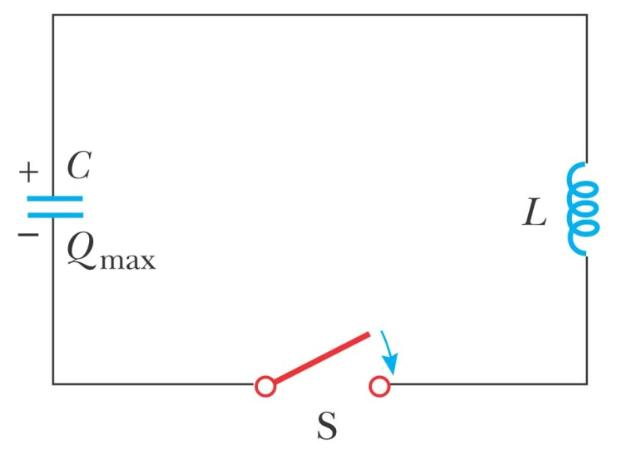
\includegraphics[scale = 0.35]{Images/Magnetisme/LCKring}
    \end{minipage}
    \vspace{-0.3cm}
    \begin{equation*}
        -L\dfrac{dI}{dt} + \dfrac{Q}{C} = 0
    \end{equation*}
    De lading op de positieve plaat, die voor de stroom zorgt, zal verminderen en dus ook de stroom. We hebben nu $I = -\tfrac{dQ}{dt}$ en we kunnen nu de bovenstaande vergelijking herwerken tot
    een differentiaalvergelijking
    \begin{equation*}
        \dfrac{d^{2}Q}{dt^{2}} + \dfrac{Q}{LC} = 0
    \end{equation*}
    wat dezelfde vorm heeft als de vergelijking van de harmonische beweging. De oplossing is dus

    \begin{minipage}{.71\textwidth}
        \begin{align*}
            Q(t) &= Q_{0}\cos(\omega t) \\
                 &= Q_{0}\cos(\tfrac{t}{\sqrt{LC}})
        \end{align*}
        \hspace{-0.6cm} en voor de stroom
        \begin{align*}
            I(t) &= -\dfrac{dQ(t)}{dt} \\
                 &= \dfrac{Q_{0}}{\sqrt{LC}}\sin(\tfrac{t}{\sqrt{LC}})
        \end{align*}
    \end{minipage}
    \begin{minipage}{.25\textwidth}
        \vspace{0.3cm}\hspace{-0.45cm}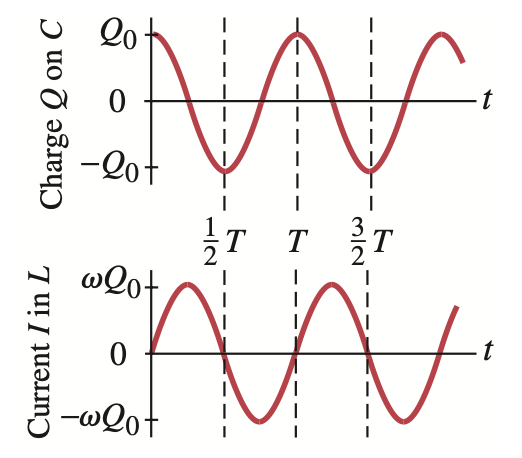
\includegraphics[scale = 0.45]{Images/Magnetisme/LCKringGrafiek}
    \end{minipage}
    We zien dat de lading en de stroom sinusvormige functies zijn van de tijd. De stroom is $90^{\circ}$ uit fase met de lading en de frequentie van de oscillaties is
    \begin{equation*}
        f = \dfrac{1}{2\pi\sqrt{LC}}
    \end{equation*}
    waaruit we $\omega = 2\pi f = \tfrac{1}{\sqrt{LC}}$ kunnen afleiden. De energie in het elektrisch veld van de condensator is

    \begin{minipage}{.70\textwidth}
        \begin{equation*}
            U_{E} = \dfrac{Q^{2}}{2C} = \dfrac{Q_{0}^2}{2C}\cos^2(\omega t)
        \end{equation*}
        \hspace{-0.6cm} en de energie in het magnetische veld van de inductor is 
        \begin{equation*}
            U_{B} = \dfrac{LI^{2}}{2} = \dfrac{LQ_{0}^2}{2C}\sin^2(\omega t)
        \end{equation*}
    \end{minipage}
    \begin{minipage}{.26\textwidth}
        \vspace{0cm}\hspace{-1.4cm}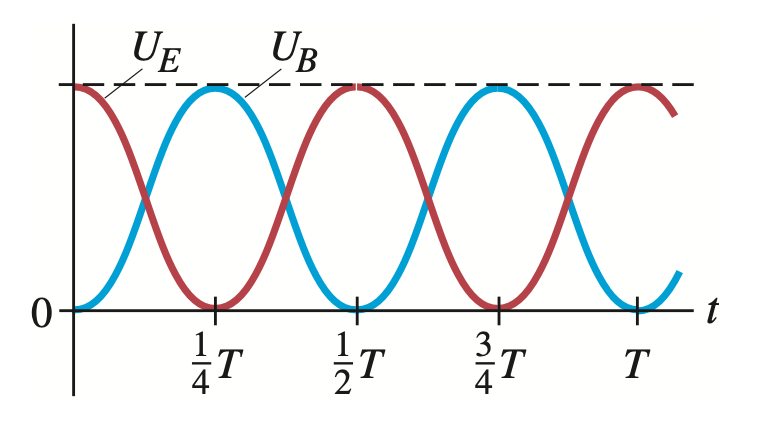
\includegraphics[scale = 0.4]{Images/Magnetisme/LCKringOscillatie.png} 
    \end{minipage}
    De totale energie in de kring is dus
    \begin{align*}
        U &= U_{E} + U_{B} \\
          &= \dfrac{Q_{0}^2}{2C}\left(\cos^2(\omega t) +\sin^2(\omega t)\right) \\ 
          &= \dfrac{Q_{0}^2}{2C}
    \end{align*}
\end{theo}

